\documentclass[aspectratio=43, xcolor=table]{beamer}
%\usepackage[english]{babel}

%Cargar paquetes
\usepackage[utf8]{inputenc}%Permite usar acentos
\usepackage[spanish]{babel}%Configura el idioma por defecto a español
\usepackage{amsmath}%Introduce términos matemáticos
\usepackage{graphicx}%Permite introducir figuras
\usepackage[options]{natbib}%Bibliografía con estilos %No funcionan estilos en Beamer
\newcommand{\grad}{\hspace{-2mm}$\phantom{a}^{\circ}$}

\usepackage{amsthm}
\usepackage{mathtools}
\usepackage{physics}
\usepackage{calligra}
\usepackage{csquotes}
\usepackage{tensor}
\usepackage[thicklines]{cancel}
\usepackage{tcolorbox}
\usepackage{pstricks}
\usepackage[backend=biber, bibstyle=nature, sorting=nty, citestyle=numeric-comp]{biblatex} %Custom bibliography
    \addbibresource{bib.bib} %Load references


\DeclareMathAlphabet{\mathcalligra}{T1}{calligra}{m}{n}
\DeclareFontShape{T1}{calligra}{m}{n}{<->s*[2.2]callig15}{}
\newcommand{\scriptr}{\mathcalligra{r}\,}
\newcommand{\boldscriptr}{\pmb{\mathcalligra{r}}\,}
\def\rc{\scriptr}
\def\brc{\boldscriptr}
\def\hrc{\hat\brc}
\newcommand{\ie}{\emph{i.e.}} %id est
\newcommand{\eg}{\emph{e.g.}} %exempli gratia
\newcommand{\rtd}[1]{\ensuremath{\left\lfloor #1 \right\rfloor}}
\newcommand{\dirac}[1]{\ensuremath{\delta \left( #1 \right)}}
\newcommand{\diract}[1]{\ensuremath{\delta^3 \left( #1 \right)}}
\newcommand{\e}{\ensuremath{\epsilon_0}}
\newcommand{\m}{\ensuremath{\mu_0}}
\newcommand{\V}{\ensuremath{\mathcal{V}}}
\newcommand{\prnt}[1]{\ensuremath{\left(#1\right)}} %parentheses
\newcommand{\colch}[1]{\ensuremath{\left[#1\right]}} %square brackets
\newcommand{\chave}[1]{\ensuremath{\left\{#1\right\}}}  %curly brackets

\useoutertheme{infolines}
\useinnertheme{rectangles}
\usefonttheme{professionalfonts}


\definecolor{orange}{HTML}{f28165}
\definecolor{gray}{HTML}{303030}
\definecolor{yellow}{HTML}{f0be52}
\definecolor{lightorange}{HTML}{f19e58}

\renewcommand{\CancelColor}{\color{orange}}

\makeatletter
\newcommand{\mybox}[1]{%
  \setbox0=\hbox{#1}%
  \setlength{\@tempdima}{\dimexpr\wd0+13pt}%
  \begin{tcolorbox}[colback=orange,colframe=orange,boxrule=0.5pt,arc=4pt,
      left=6pt,right=6pt,top=6pt,bottom=6pt,boxsep=0pt,width=\@tempdima]
    \textcolor{white}{#1}
  \end{tcolorbox}
}
\makeatother

\usecolortheme[named=orange]{structure}
\usecolortheme{sidebartab}
\usecolortheme{orchid}
\usecolortheme{whale}
\setbeamercolor{alerted text}{fg=yellow}
\setbeamercolor{block title alerted}{bg=alerted text.fg!90!black}
\setbeamercolor{block title example}{bg=lightorange!60!black}
\setbeamercolor{background canvas}{bg=gray}
\setbeamercolor{normal text}{bg=gray,fg=white}

\setbeamertemplate{footline}
        {
      \leavevmode%
      \hbox{%
      \begin{beamercolorbox}[wd=.333333\paperwidth,ht=2.25ex,dp=1ex,center]{author in head/foot}%
        \usebeamerfont{author in head/foot}\insertshortauthor~~(\insertshortinstitute)
      \end{beamercolorbox}%
      \begin{beamercolorbox}[wd=.333333\paperwidth,ht=2.25ex,dp=1ex,center]{title in head/foot}%
        \usebeamerfont{title in head/foot}\insertshorttitle
      \end{beamercolorbox}%
      \begin{beamercolorbox}[wd=.333333\paperwidth,ht=2.25ex,dp=1ex,center]{date in head/foot}%
        \usebeamerfont{page number in head/foot}\insertframenumber/\inserttotalframenumber%\hspace*{2em}

    %#turning the next line into a comment, erases the frame numbers
        %\insertframenumber{} / \inserttotalframenumber\hspace*{2ex} 

      \end{beamercolorbox}}%
      \vskip0pt%
    }


\setbeamertemplate{blocks}[rectangle]
\setbeamercovered{dynamic}

\setbeamertemplate{section page}
{
	\begin{centering}
		\begin{beamercolorbox}[sep=27pt,center]{part title}
			\usebeamerfont{section title}\insertsection\par
			\usebeamerfont{subsection title}\insertsubsection\par
		\end{beamercolorbox}
	\end{centering}
}

%\setbeamertemplate{subsection page}
%{
%	\begin{centering}
%		\begin{beamercolorbox}[sep=12pt,center]{part title}
%			\usebeamerfont{subsection title}\insertsubsection\par
%		\end{beamercolorbox}
%	\end{centering}
%}

\newcommand{\hlight}[1]{\colorbox{violet!50}{#1}}
\newcommand{\hlighta}[1]{\colorbox{red!50}{#1}}
\title{Generación de números aleatorios} %->->->->-> Check hyperref title <-<-<-<-<-
%\subtitle{And Some Things About It}
\author[C.J. Uribe-Martes]{Carlos Javier Uribe Martes}
\institute[CUC]{
    Ingeniería Industrial%
    \\%
    Universidad de la Costa%
} %You can change the Institution if you are from somewhere else
\date{Febrero 11, 2020}
%\logo{\includegraphics[width= 0.2\textwidth]{images/a-logo.png}}

\begin{document}
    
    \frame{\titlepage}
    
    \begin{frame}{Contenido}
        \tableofcontents
    \end{frame}
    
    \section[Propiedades]{Propiedades de los números aleatorios}
\begin{frame}{Introducción}
    \begin{itemize}
        \item Para desarrollar un modelo de simulación el ingrediente fundamental es la generación de una secuencia de números aleatorios $R_1, R_2, \dots , R_n$ \cite{BCN}.
        %\item La mayoría de los lenguajes de computador tienen una subrutina, objecto o función capaz de generar números aleatorios \cite{BCN}.
    \end{itemize}
\end{frame}

\begin{frame}{Propiedades de los números aleatorios}
    \begin{itemize}
        %\item Una secuencia de números aleatorios $R_1, R_2, \dots$, debe tener dos propiedades estadísticas importantes: uniformidad e independencia \cite{BCN}.
        
        \item Cada número aleatorio $R_i$ debe ser una muestra \textit{independiente} obtenida de una distribución \textit{uniforme} continua entre cero y uno \cite{BCN}.
        
    \end{itemize}
\end{frame}

\begin{frame}{Propiedades de la distribución uniforme $\left[0,1\right]$}
    $\begin{array}{ccc}
        f(x)=\left\{\begin{array}{cl}
        1, & 0\leq x \leq 1  \\
        0, & \text{de lo contrario}
    \end{array}\right.; & E(R)=\frac{1}{2}; & V(R)=\frac{1}{12}
    \end{array}$
    %\vskip-4pt
    \begin{columns}
        \begin{column}{0.5\textwidth}
            \begin{figure}
                \centering
                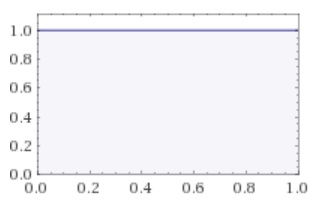
\includegraphics[width=5cm]{images/uniform_pdf.jpg}
                \caption{Función de densidad de probabilidad}
                \label{fig:pdf}
            \end{figure}
        \end{column}
        \begin{column}{0.5\textwidth}
            \begin{figure}
                \centering
                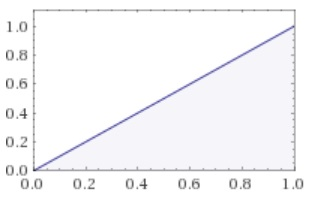
\includegraphics[width=5cm]{images/uniform_cdf.jpg}
                \caption{Función de probabilidad acumulada}
                \label{fig:cdf}
            \end{figure}
        \end{column}
    \end{columns}
\end{frame}

    
    \section[Técnicas de generación]{Técnicas de generación de números aleatorios}

\begin{frame}{Generación de números pseudo-aleatorios}
    \begin{itemize}
        \item Generar números aleatorios a través de un algoritmo  remueve la verdadera aleatoriedad, toda vez que el patrón puede ser repetido \cite{BCN}.
        %\item De allí que se hable de números \textit{pseudo-aleatorios}.
        \item Se busca generar una secuencia de números que \textit{imite} las propiedades de los números aleatorios  \cite{BCN}.
    \end{itemize}
\end{frame}

\begin{frame}{Técnicas para generación de números aleatorios}
    \begin{itemize}
        \item Una técnica adecuada debe tener las siguientes características:
            \begin{itemize}
                \item Eficiencia \cite{PSD}.
                \item Periodo máximo \cite{PSD}.
                \item Secuencia reproducible \cite{PSD}.  
                \item Portabilidad \cite{LK}.
            \end{itemize}
    \end{itemize}

\end{frame}

\begin{frame}{Cuadrados medios de Von Neumann y Metropolis}
    %Fue propuesto en la década de los años cuarenta del siglo XX por Von Neumann y Metropolis. Requiere una semila $X_0$, la cual es elevada al cuadrado para seleccionar los $D$ dígitos del centro. El método es el siguiente:
    \begin{enumerate}
        \item Seleccione una \textit{semilla} $X_0$ con $D$ dígitos ($D>3$).
        \item Sea $Y_0$ el resultado de elevar $X_0$ al cuadrado, defina $X_1$ igual a los $D$ dígitos del centro de $Y_0$ y sea $R_1=0.X_1$.
        \item Sea $Y_i$ el resultado de elevar $X_i$ al cuadrado, defina $X_{i+1}$ igual a los $D$ dígitos del centro de $Y_i$ y sea $R_{i+1}=0.X_{i+1}$.
        %\item Repita el paso 3 hasta obtener los $n$ números $R_i$ deseados.
    \end{enumerate}
    
    %Si en algún punto no es posible obtener los $D$ dígitos del centro del número $Y_i$, agregue ceros a la izquierda de éste.
\end{frame}

\begin{frame}{Generador congruencial lineal}
        \begin{itemize}
        \item Utiliza la siguiente relación recursiva \begin{equation*}
            X_{i+1}=\left(aX_i+c\right)\mod m, \quad i=0,1,2,\dots
        \end{equation*}
        %\item Produce una secuencia de enteros $X_1, X_2, \dots$ entre 0 y $m-1$ siguiendo la relación recursiva \begin{equation*}
        %    X_{i+1}=\left(aX_i+c\right)\mod m, \quad i=0,1,2,\dots
        %\end{equation*}
        \item El valor inicial $X_0$ es llamado \textit{semilla}, $a$ es el \textit{multiplicador}, $c$ es el \textit{incremento} y $m$ el \textit{módulo}, todos enteros no negativos.
        \item Para obtener $R_i$ emplee:
        \begin{equation*}R_i=\frac{X_i}{m}, \quad i=1,2,\dots\end{equation*}
    \end{itemize}
\end{frame}

\begin{frame}{Generador congruencial lineal}
    
    \begin{itemize}
        \item Los valores de $a, c, m$ y $X_0$ afectan directamente las propiedades estadísticas y el periodo de la secuencia generada \cite{BCN}.
        \item Deben satisfacerse las siguientes relaciones:
        \begin{itemize}
            \item $a < m$
            \item $c < m$
            \item $m > 0$
            \item $X_0 < m$
        \end{itemize}
        \item La secuencia se repetirá con periodo $p\leq m$, por lo que el generador alcanza el periodo máximo cuando $p=m$
    \end{itemize}
\end{frame}

%\begin{frame}{Generadores congruenciales lineales}
%    \begin{block}{Actividad en clase}{Use el método de congruencial lineal para generar una secuencia de números aleatorios definiendo una semilla, un multiplicador y un incremento, considerando un módulo $m=100$. Determine la longitud del ciclo de la secuencia generada.} 
%    \end{block}
%\end{frame}

%\begin{frame}{Generadores congrenciales mixtos}
%    \begin{itemize}
%        \item Las condiciones siguientes aseguran que el generador congruencial mixto que las satisfaga tendrá periodo máximo \cite{PSD, LK}:
%        \begin{enumerate}
%            \item El único entero positivo que divide exactamente a $m$ y a $c$ es 1, es decir, son primos entre sí.
%            \item Si $q$ es un número primo que divide a $m$, entonces $q$ también divide a $a-1$.
%            \item Si 4 divide a $m$, entonces 4 también divide a $a-1$.
%        \end{enumerate}
%    \end{itemize}
%\end{frame}

%\begin{frame}{Generadores congrenciales mixtos}
%    En la siguiente tabla se indican los generadores congruenciales lineales mixtos propuestos por Coveyou y MacPherson (1967) y por Kobayashi (1978) \cite{PSD}.
%    \begin{table}[]
%    \begin{tabular}{|l|l|l|}
%    \hline
%    \textbf{Parámetros} & \textbf{Kobayashi} & \textbf{\begin{tabular}[c]{@{}l@{}}Coveyou y\\ MacPherson\end{tabular}} \\ \hline
%    $a$ & 314.159.269 & $5^15$ \\ \hline
%    $c$ & 453.806.245 & 1 \\ \hline
%    $m$ & $2^{31}$ & $2^{35}$ \\ \hline
%    \end{tabular}
%    \end{table}
%\end{frame}

%\begin{frame}{Generadores congruenciales lineales}
%    \begin{itemize}
%        
%        \item Por máxima densidad se entiende que los valores asumidos por $R_i, i=1,2,\dots$ no dejen vacíos largos en el intervalo $[0,1]$.
%        \item Para alcanzar la máxima densidad y evitar ciclos (la recurrencias de la misma secuencia de números generados), el generador debe tener el periodo más largo posible.
%    \end{itemize}
%\end{frame}

\begin{frame}{Generador congruencial multiplicativo}
    \begin{itemize}
        \item Si el incremento $c=0$, se denomina \textit{método congruencial multiplicativo}.
        \item No alcanza el periodo máximo ya que la secuencia no contendrá $X_i=0$, sin embargo pueden llegar a alcanzar el periodo $m-1$ si se seleccionan $m$ y $a$ en forma adecuada \cite{PSD}:
        \begin{itemize}
            \item $m$ ha de ser un número primo.
            \item $a$ ha de ser raíz primitiva de $m$, es decir, \begin{equation*}a^n \mod m \neq 1 \quad n=1,\dots, m-2\end{equation*}
        \end{itemize}
    \end{itemize}
\end{frame}

\begin{frame}{Generador congruencial multiplicativo}
    \begin{itemize}
    \item La siguiente tabla indica los parámetros evaluados por Fishman y Moore (1986) que tienen buen comportamiento \cite{PSD}.
% Please add the following required packages to your document preamble:
% \usepackage[table,xcdraw]{xcolor}
% If you use beamer only pass "xcolor=table" option, i.e. \documentclass[xcolor=table]{beamer}
    \begin{table}[]
    \begin{tabular}{|c|r|}
    \hline
    \rowcolor[HTML]{794033} 
    {\color[HTML]{FFFFFF} \textbf{Parámetros}} & {\color[HTML]{FFFFFF} \textbf{Fishman y Moore}} \\ \hline
    \rowcolor[HTML]{F28165} 
    a & 48.271\\ \hline
    \rowcolor[HTML]{F28165} 
    m & $2^{31}-1$ \\ \hline
    \end{tabular}
    \end{table}
    \end{itemize}
\end{frame}

\begin{frame}{Generador congrencial mixto}
    \begin{itemize}
        \item Si el incremento $c\neq 0$, se denomina \textit{método congruencial mixto}. 
        \item Las siguientes condiciones aseguran que el generador congruencial mixto tendrá periodo máximo \cite{PSD, LK}:
        \begin{enumerate}
            \item El único entero positivo que divide a $m$ y a $c$ es 1, es decir, son primos entre sí.
            \item Si $q$ es un número primo que divide a $m$, entonces $q$ también divide a $a-1$.
            \item Si 4 divide a $m$, entonces 4 también divide a $a-1$.
        \end{enumerate}
    \end{itemize}
\end{frame}

\begin{frame}{Generadores congrenciales mixtos}
    \begin{itemize}
    \item La siguiente tabla indica los generadores congruenciales lineales mixtos propuestos por Coveyou y MacPherson (1967) y por Kobayashi (1978) \cite{PSD}.
% Please add the following required packages to your document preamble:
% \usepackage[table,xcdraw]{xcolor}
% If you use beamer only pass "xcolor=table" option, i.e. \documentclass[xcolor=table]{beamer}
    \begin{table}[]
    \begin{tabular}{|c|r|r|}
    \hline
    \rowcolor[HTML]{794033} 
    {\color[HTML]{FFFFFF} \textbf{Parámetros}} & {\color[HTML]{FFFFFF} \textbf{Kobayashi}} & {\color[HTML]{FFFFFF} \textbf{Coveyou y MacPherson}} \\ \hline
    \rowcolor[HTML]{F28165} 
    a & 314.159.269 & $5^{15}$ \\ \hline
    \rowcolor[HTML]{F28165} 
    c & 453.806.245 & 1 \\ \hline
    \rowcolor[HTML]{F28165} 
    m & $2^{31}$ & $2^{35}$ \\ \hline
    \end{tabular}
    \end{table}
    \end{itemize}
\end{frame}


\begin{frame}{Métodos congruenciales NO lineales}
    \begin{itemize}
        \item \textbf{Algoritmo congruencial cuadrático}: Emplea la relación recursiva: \begin{equation*}
            X_{i+1}=\left(aX_i^2+bX_i+c\right)\mod m, \quad i=0,1,2,\dots
        \end{equation*}
        \item \textbf{Algoritmo de Blum, Blum y Shub}: Es similar al algoritmo congruencial cuadrático, con $a=1, b=0, c=0$, entonces la relación recursiva es:
        \begin{equation*}
            X_{i+1}=X_i^2\mod m, \quad i=0,1,2,\dots
        \end{equation*}
    \end{itemize}
\end{frame}


\begin{frame}{Combinación de generadores congruenciales lineales}
    \begin{itemize}
        \item Una manera de conseguir secuencias aleatorias con periodos más largos es combinar dos o más generadores congruenciales multiplicativos.
    \end{itemize}
\end{frame}

\begin{frame}{Generador de Wichmann-Hill}
    \begin{itemize}
        \item Consiste en tres generadores congruenciales lineales con módulos primos. Cada uno es utilizado para producir un aleatorio entre 0 y 1.  
        \item Estos tres resultados se suman, módulo 1, para obtener el resultado final.
        %\item El algoritmo es el siguiente:
        \begin{enumerate}
            \item $x_i=171 x_{i-1} \mod 30269$
            \item $y_i=172 y_{i-1} \mod 30307$
            \item $z_i=170 z_{i-1} \mod 30323$
            \item $r_i=\left(\dfrac{x_i}{30269}+\dfrac{y_i}{30307}+\dfrac{z_i}{30323}\right)\mod 1$
        \end{enumerate}
    \end{itemize}

\end{frame}

\begin{frame}{MRG32k3a de L'Ecuyer}
    \begin{itemize}
        \item Consiste en dos generadores congruenciales recursivos de tercer orden.
        \item Estos se combinan para obtener un nuevo aleatorio en cada iteración.
        %\item El algoritmo es el siguiente:
        \begin{enumerate}
        \item $x_i=\left(1403580 x_{i-2}-810728 x_{i-3}\right) \mod \left(2^{32}-209\right)$
        \item $y_i=\left(527612 y_{i-1}-1370589 y_{i-3}\right) \mod \left(2^{32}-22853\right)$
        \item $z_i=\left(x_{i}-y_{i}\right) \mod \left(2^{32}-209\right)$
        \item $r_i=\dfrac{z_i}{2^{32}-209}$
    \end{enumerate}
    \end{itemize}


\end{frame}
    
    \section[Pruebas estadísticas]{Pruebas estadísticas para números aleatorios}

\begin{frame}{Pruebas para números aleatorios}
    \begin{itemize}
        \item Para verificar si las propiedades deseadas de un conjunto de números aleatorios diferentes tipos de pruebas pueden desarrollarse.
        \item Para cada prueba debe definirse un nivel de significancia $\alpha$, el cual representa la probabilidad de rechazar la hipótesis nula cuando ésta es cierta:
        \begin{equation*}
            \alpha=P(\text{rechazar }H_0|H_0\text{ es cierta})
        \end{equation*}
        
        %\item El analista define este valor para cada prueba. Algunos valores comunes de $\alpha$ son 0.01 y 0.05.
    \end{itemize}
\end{frame}

\subsection{Pruebas de uniformidad}

\begin{frame}{Prueba de medias}
    \begin{itemize}
        \item Busca comprobar que el valor esperado de los números en la secuencia $R_i$ sea igual a 0.5 mediante las siguientes hipótesis: 
                \begin{eqnarray*}
                    H_0:~\mu_{R_i} = 0.5\\
                    H_1:~\mu_{R_i} \neq 0.5
                \end{eqnarray*}
    \end{itemize}
\end{frame}

\begin{frame}{Prueba de medias}
    %El algoritmo para la prueba de medias es el siguiente:
    \begin{enumerate}
        \item Determine el promedio de los $n$ números aletorios de la secuencia: 
        \begin{equation*}
            \bar{R}=\frac{1}{n} \sum_{i=1}^{n}{R_i}
        \end{equation*}
        \item Calcule los límites de aceptación inferior y superior: 
                \begin{eqnarray*}
                    LI_{\bar{R}}=\frac{1}{2}-z_{\alpha/2}\left(\frac{1}{\sqrt{12n}}\right)\\
                    LS_{\bar{R}}=\frac{1}{2}+z_{\alpha/2}\left(\frac{1}{\sqrt{12n}}\right)
                \end{eqnarray*}
        \item Si el valor de $\bar{R}$ está dentro de los límites de aceptación no hay evidencia suficiente para rechazar $H_0$ con un nivel de confianza 1-$\alpha$. 
    \end{enumerate}
\end{frame}

\begin{frame}{Prueba de varianza}
    \begin{itemize}
        \item Busca determinar si la varianza de la secuencia aleatoria generada es igual a 1/12 mediante las siguientes hipótesis:
            \begin{eqnarray*}
                H_0:~\sigma^2_{R_i} = \frac{1}{12}\\
                H_1:~\sigma^2_{R_i} \neq \frac{1}{12}
            \end{eqnarray*}        
    \end{itemize} 
\end{frame}

\begin{frame}{Prueba de varianza}
    %La prueba de varianza tiene los siguientes pasos:
    \begin{enumerate}
        \item Determine la varianza muestral de la secuencia $R_1, R_2, \dots, R_n$: \begin{equation*}
            V(R)=\frac{\displaystyle{\sum_{i=1}^{n}{(R_i-\bar{R})^2}}}{n-1}
        \end{equation*}
        \item Calcule los límites de aceptación inferior y superior mediante: 
                \begin{eqnarray*}
                    LI_{V(R)}=\frac{\chi^2_{\frac{\alpha}{2},n-1}}{12(n-1)}\\
                    LS_{V(R)}=\frac{\chi^2_{\frac{(1-\alpha)}{2},n-1}}{12(n-1)}
                \end{eqnarray*}
        \item Si el valor de $V(R)$ está dentro de los límites de aceptación no hay evidencia suficiente para rechazar $H_0$ con un nivel de confianza 1-$\alpha$. 
    \end{enumerate}
\end{frame}

\begin{frame}{Prueba de frecuencias}
    \begin{itemize}
        \item Trata de determinar si el conjunto de números generados se distribuye de acuerdo con la distribución uniforme $\left[0,1\right]$ para lo cual formula las siguientes hipótesis:
        \begin{eqnarray*}
            H_0:~R_i \sim U\left[0,1\right]\\
            H_1:~R_i \not\sim U\left[0,1\right]
        \end{eqnarray*}
        %\item Utiliza la prueba chi-cuadrado o Kolmogorov-Smirnov para comparar la distribución del conjunto de números generados con la distribución uniforme.
    \end{itemize}
\end{frame}

\begin{frame}{Prueba de frecuencias}{Prueba chi-cuadrado}
    \begin{itemize}
        \item Para la distribución uniforme, la frecuencia esperada en cada clase, $E_i$ está dada por: 
        \begin{equation*}
            E_i=\frac{N}{n}
        \end{equation*}
       para  $n$ clases igualmente espaciadas, donde $N$ es el número total de observaciones.
        \item Utiliza el estadístico de prueba:
    \begin{equation*}
        \chi_0^2=\sum_{i=1}^{n}{\frac{\left(O_i-E_i\right)^2}{E_i}}
    \end{equation*}
    donde $O_i$ es la frecuencia observada en la $i$-ésima clase. 
    \end{itemize}
\end{frame}

\begin{frame}{Prueba de frecuencias}{Prueba chi-cuadrado}
    \begin{itemize}
        \item La distribución muestral de $\chi_0^2$ es aproximadamente chi-cuadrado con $n-1$ grados de libertad.
        \item Si el estadístico de prueba $\chi_0^2$ es menor que el valor $\chi_{\alpha,n-1}^2$ no hay evidencia suficiente para rechazar $H_0$ con un nivel de confianza 1-$\alpha$.
    \end{itemize}
\end{frame}

\begin{frame}{Prueba de frecuencias}{Prueba Kolmogorov-Smirnov}
    \begin{itemize}
        \item Contrasta la función de densidad acumulada $F(x)$ de la distribución teórica con la función de densidad empírica $S_N(x)$ de la muestra de $N$ obsevaciones.
        \item Se basa en la mayor desviación absoluta entre $F(x)$ y $S_N(x)$ en el rango de la variable aleatoria, utilizando el estadístico de prueba:
        \begin{equation*}
            D=max |F(x)-S_N(x)|
        \end{equation*}
    \end{itemize}
\end{frame}

\begin{frame}{Prueba de frecuencias}{Prueba Kolmogorov-Smirnov}
    \begin{enumerate}
        \item Ordene los datos de menor a mayor. Sea $R_{(i)}$ la $i$-ésima menor observación.
        \item Determine los valores:
            \begin{eqnarray*}
                D^+=max_{1\leq i \leq N} \left\{\frac{i}{N}-R_{(i)}\right\} \\
                D^-=max_{1\leq i \leq N} \left\{R_{(i)} - \frac{i-1}{N}\right\}
            \end{eqnarray*}
        \item Calcule $D=max(D^+,D^-)$.
        \item Identifique el valor crítico $D_{\alpha}$ correspondiente a $\alpha$ y $N$. Esta valor se puede encontrar en las tablas estadísticas de Kolmogorov-Smirnov.
        \item Si $D\leq D_{\alpha}$ se concluye que no hay evidencia suficiente para rechazar $H_0$ con un nivel de confianza 1-$\alpha$.
    \end{enumerate}
\end{frame}

\subsection{Pruebas de independencia}

\begin{frame}{Pruebas de independencia}
    En su mayoría buscan probar la independencia de los números de un conjunto $R_i$ mediante las hipótesis:
        \begin{eqnarray*}
            H_0:~\text{los números del conjunto $R_i$ son independientes}\\
            H_1:~\text{los números del conjunto $R_i$ no son independientes}
        \end{eqnarray*}
\end{frame}

\begin{frame}{Prueba de corridas arriba y abajo}
    \begin{enumerate}
        \item Determine una secuencia de unos y ceros así: si $R_{i+1}\leq R_i$ asigne un cero a la secuencia, de lo contrario asigne un uno.
        \item Defina $C_0$ como el número de corridas en la secuencia (una corrida es cualquier cantidad de unos o ceros consecutivos).
        \item Determine el estadístico de prueba mediante las ecuaciones:
            \begin{eqnarray*}
                \mu_{C_0}=\frac{2n-1}{3} \\
                \sigma^2_{C_0}=\frac{16n-29}{90}\\
                Z_0=\left|\frac{C_0-\mu_{C_0}}{\sigma_{C_0}}\right|
            \end{eqnarray*}
        \item Si el estadístico $Z_0$ es mayor que el valor crítico de $Z_{\alpha/2}$, se concluye que los números del conjunto $R_i$ no son independientes.
    \end{enumerate}
\end{frame}

\begin{frame}{Prueba de corridas arriba y abajo de la media}
    \begin{enumerate}
        \item Determine una secuencia de unos y ceros así: si $R_{i}\leq 0.5$ asigne un cero a la secuencia, de lo contrario asigne un uno.
        \item Defina $C_0$ como el número de corridas en la secuencia, $n_0$ el número de ceros de ceros y $n_1$ el número de unos.
        \item Determine el estadístico de prueba mediante las ecuaciones:
            \begin{eqnarray*}
                \mu_{C_0}=\frac{2n_0n_1}{n}+0.5 \\
                \sigma^2_{C_0}=\frac{2n_0n_1(2n_0n_1-n)}{n^2(n-1)}\\
                Z_0=\frac{C_0-\mu_{C_0}}{\sigma_{C_0}}
            \end{eqnarray*}
        \item Si el estadístico $Z_0$ está fuera del intervalo $\left[-Z_{\alpha/2}, Z_{\alpha/2}\right]$ se concluye que los números del conjunto $R_i$ no son independientes.
    \end{enumerate}
\end{frame}

%PRUEBA DE POKER GARCIA DUNNA pag 56
%PRUEBA DE SERIES
%PRUEBA DE HUECOS

\begin{frame}{Prueba de autocorrelación}
    \begin{itemize}
        \item Prueba la correlación entre los números generados y compara la correlación muestral con la correlación esperada de cero.
        
        \item Requiere el cálculo de la autocorrelación entre cada $m$ números (siendo conocida $m$ como \textit{lag} o retraso), empezando con el $i$-ésimo número de la secuencia.
        
        \item La autocorrelación $\rho_{im}$  entre los siguientes números será de interés $R_i$, $R_{i+m}, R_{i+2m},\dots, R_{i+(M+1)m}$. Donde el valor de $M$ es el entero más grande tal que $i+(M+1)m\leq N$,

    \end{itemize}
    
\end{frame}

\begin{frame}{Prueba de autocorrelación}
    \begin{itemize}
        \item Una autocorrelación diferente de cero implica una falta de independencia en los datos. La siguiente prueba con dos colas es adecuada:
        \begin{eqnarray*}
            H_0:~\rho_{im} = 0\\
            H_1:~\rho_{im} \neq 0
        \end{eqnarray*}
        \item Para valores grandes de $M$, la distribución del estimador de $\rho_{im}$, denotado $\hat{\rho}_{im}$, es aproximadamente normal si los valores $R_i$, $R_{i+m}, R_{i+2m},\dots, R_{i+(M+1)m}$ no están correlacionados. 
        
    \end{itemize}
    
\end{frame}

\begin{frame}{Prueba de autocorrelación}
    \begin{itemize}

        \item El estadístico: 
        \begin{equation*}
            Z_0=\frac{\hat{\rho}_{im}}{\sigma_{\hat{\rho}_{im}}}
        \end{equation*}
        está normalmente distribuido con media 0 y varianza 1, bajo el supuesto de independencia y para valores grandes de $M$.
        
        \item Donde \begin{eqnarray*}
            \hat{\rho}_{im}&=&\frac{1}{M+1}\left[\sum_{k=0}^{M}{R_{i+km}R_{i+(k+1)m}}\right]-0.25\\
            \sigma_{\hat{\rho}_{im}}&=&\frac{\sqrt{13M+7}}{12(M+1)}
        \end{eqnarray*}
        
        \item No rechace $H_0$ si $-z_{\alpha/2}\leq Z_0 \leq z_{\alpha/2}$ donde $z_{\alpha/2}$ se puede obtener de la tabla de probabilidades para la distribución chi-cuadrado.
    \end{itemize}
    
\end{frame}

%\begin{frame}{Frame Title}
%    t_0=\dfrac{\bar{y_1}-\bar{y_2}}{S_p\sqrt{\dfrac{1}{n_1}+\dfrac{1}{n_2}}}
%\end{frame}
    
    \section*{Referencias} %You can remove this if you do not want to use it
        \begin{frame}{Referencias}
            \printbibliography
        \end{frame}
     
    \section{}   
        \begin{frame}{}
            \begin{figure}
                \centering
                
\includegraphics[width=6cm]{images/model.png}
                %\caption{Caption}
                %\label{fig:my_label}
            \end{figure}
        \end{frame}

\end{document}
